\section{Resultados}
%Deben incluir los resultados de los experimentos, utilizando el formato más adecuado
%para su presentación. Deberón especificar claramente a qué experiencia corresponde
%cada resultado. No se incluirán aquí corridas de máquina. Algo fundamental en su
%aprendizaje en la materia es la presentación de resultados de forma clara y concisa para
%el lector.



\subsection{Experimento 1}
Se procedió a ejecutar el método de kNN variando k, para K = 2, 10 y 20 con k $\in$ $\{$2, 30, 100, 500$\}$ .

Se observo que la memoria utilizada por el programa era de 127,6 Mb en sus fases iniciales, hasta que en un punto se queda en 380,5 Mb.

Los resultados obtenidos fueron los siguientes:
\begin{itemize}
\item Con K = 2\\
\end{itemize}

\begin{table}[H]
\centering
\begin{tabular}{|r|r|r|}
\hline
\multicolumn{1}{|c|}{k} & \multicolumn{1}{c|}{Tiempo} & \multicolumn{1}{c|}{Tasa} \\ \hline
2 & 15941.152 & 0.952476 \\ \hline
30 & 19450.181 & 0.942452 \\ \hline
100 & 19116.135 & 0.91681 \\ \hline
500 & 20496.988 & 0.844905 \\ \hline
\end{tabular}
\caption{Tasas para Knn variando k para dos particiones}
\label{}
\end{table}

\bigskip
\bigskip
\bigskip

    \begin{figure}[H]
    \centering
    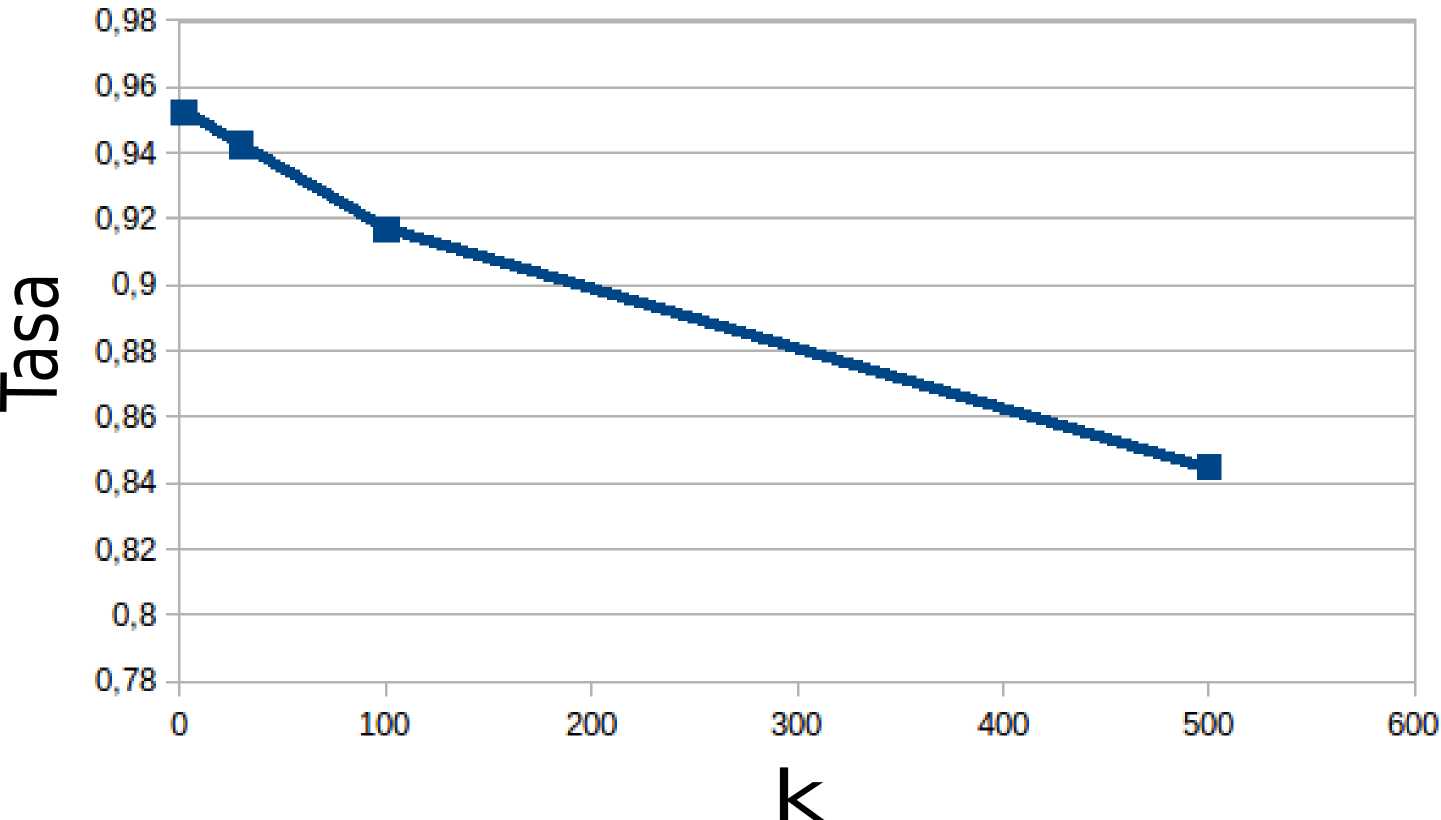
\includegraphics[scale=0.3]{Graficos/knnTasa2.png}
    \caption{Tasas para Knn variando k para dos particiones}
	\label{knnTasa2}
    \end{figure}
\bigskip
\bigskip
\bigskip






\begin{itemize}
\item Con K=10\\
\end{itemize}

\begin{center}

\begin{table}[H]
\centering
\begin{tabular}{|r|r|r|}
\hline
%\multicolumn{ 3}{|c|}{kNN variando k con K = 10} \\ \hline
\multicolumn{1}{|c|}{k} & \multicolumn{1}{c|}{Tiempo} & \multicolumn{1}{c|}{Tasa} \\ \hline
2 & 31056.21 & 0.96169 \\ \hline
30 & 34590.4  & 0.952262 \\ \hline
100 & 34449.695 & 0.93169 \\ \hline
500 & 37274.029 & 0.878833 \\ \hline
\end{tabular}
\caption{Resultados para Knn variando k para diez particiones}
\label{}
\end{table}
\end{center}

\bigskip
\bigskip
\bigskip

    \begin{figure}[H]
    \centering
    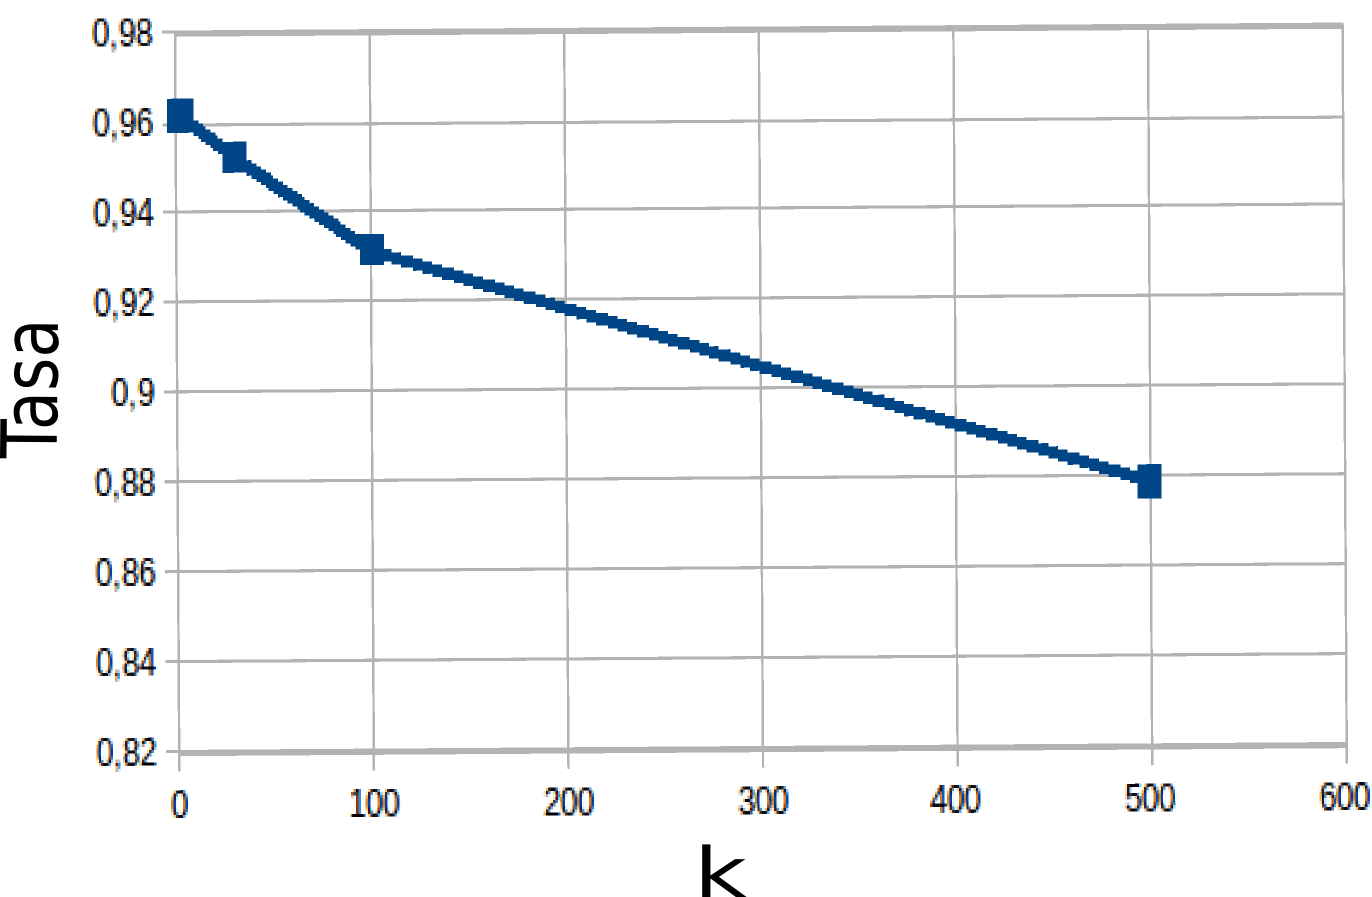
\includegraphics[scale=0.3]{Graficos/knnTasa10.png}
    \caption{Tasas para Knn variando k para diez particiones}
	\label{knnTasa10}
    \end{figure}
\bigskip
\bigskip
\bigskip




\begin{itemize}
\item Con K = 20\\
\end{itemize} 

\begin{table}[H]
\centering
\begin{tabular}{|r|r|r|}
\hline
\multicolumn{1}{|c|}{k} & \multicolumn{1}{c|}{Tiempo} & \multicolumn{1}{c|}{Tasa} \\ \hline
2 & 238893.923 & 0.962381 \\ \hline
30 & 263245.053 & 0.953167 \\ \hline
100 & 284027.496 & 0.933429 \\ \hline
500 & 313345.443 & 0.881381 \\ \hline
\end{tabular}
 \caption{Tasas para Knn variando k para veinte particiones}
\label{}
\end{table}
\bigskip
\bigskip
\bigskip

    \begin{figure}[H]
    \centering
    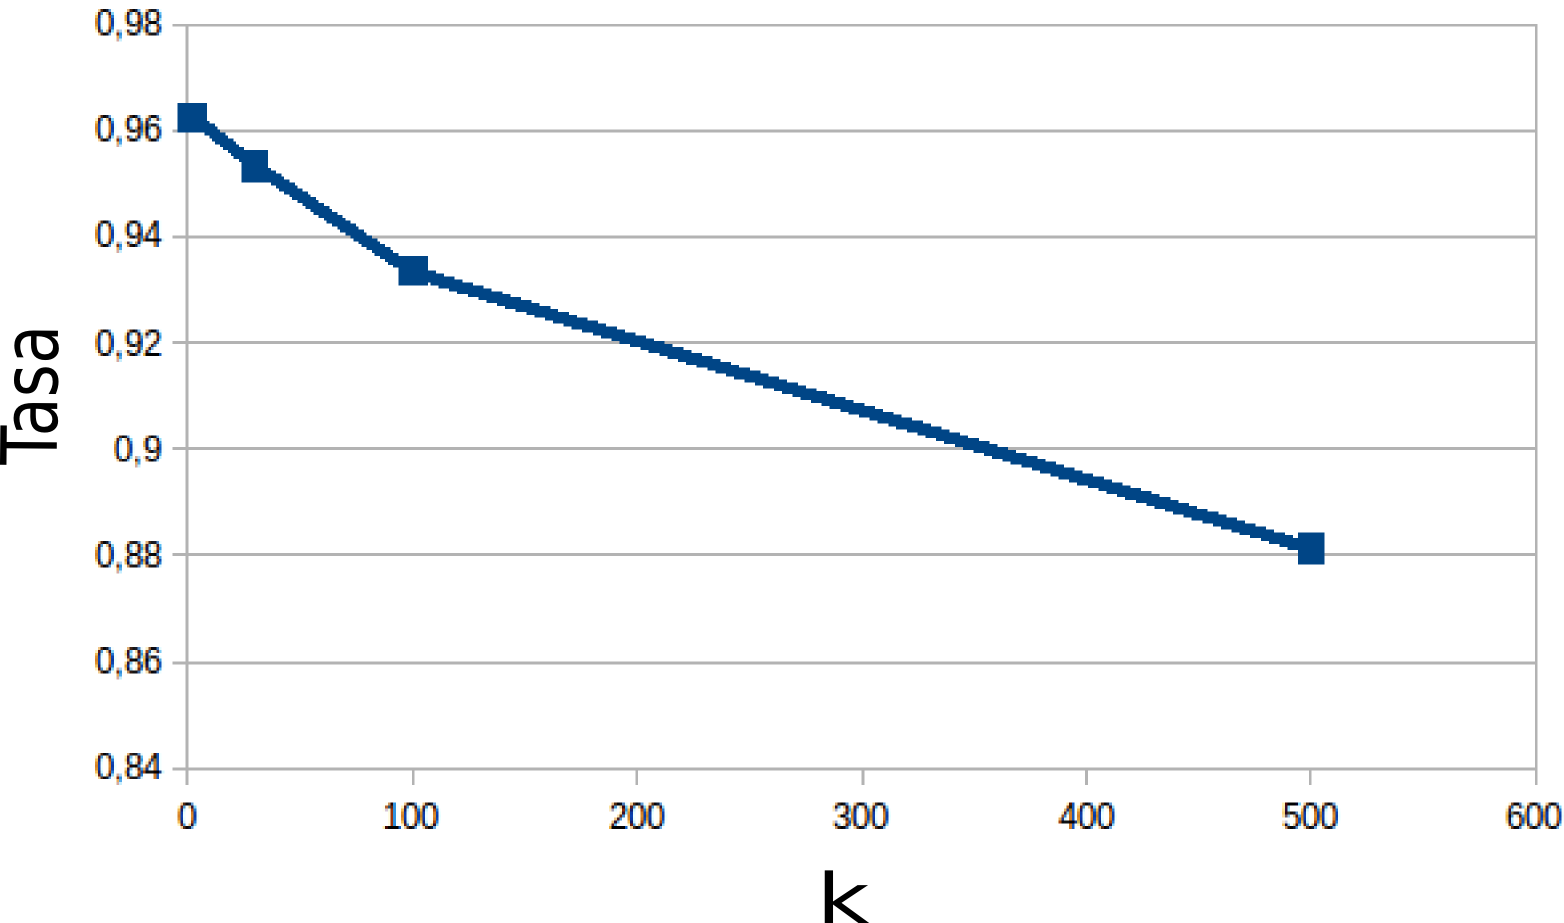
\includegraphics[scale=0.3]{Graficos/knnTasa20.png}
    \caption{Tasas para Knn variando k para veinte particiones}
	\label{knnTasa20}
    \end{figure}
\bigskip
\bigskip

En base a estos resultados se puede apreciar claramente la caída de la tasa en función de la cantidad de vecinos mas cercanos(k), y el aumento de tiempo con el mismo.

\subsection{Experimento 2}
\subsubsection{Variando k}
A continuación, presentamos las tablas correspondientes a las tasas de reconocimiento y el tiempo de cómputo para los valores de $k$ elegidos en el desarrollo y para los distintos valores de $K$:
\newline
\newline
\centerline{Tasas:}
\newline
\centerline{
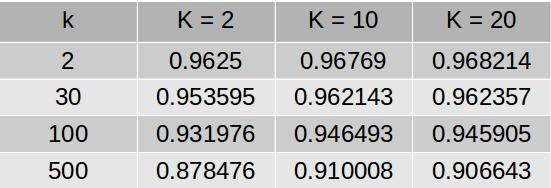
\includegraphics[scale=0.4]{Tablas/variandoktr.jpg}
}
\newline
\newline
\centerline{Tiempos:}
\newline
\centerline{
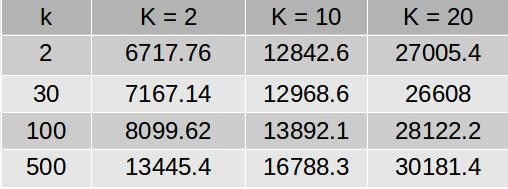
\includegraphics[scale=0.4]{Tablas/variandok.jpg}
}
\newline
\newline
Ahora vamos a comparar las tasas de PCA + KNN con las de KNN para los distintos $K$:
\newline
\newline
\centerline{
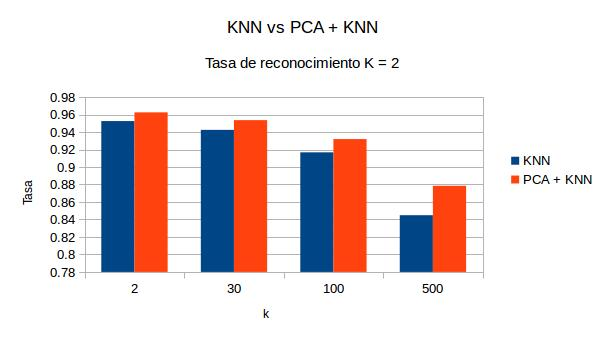
\includegraphics[scale=0.5]{Tablas/comtrK2.jpg}
}
\centerline{
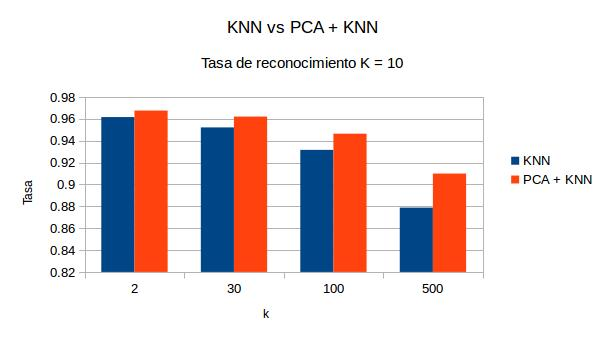
\includegraphics[scale=0.5]{Tablas/comtrK10.jpg}
}
\centerline{
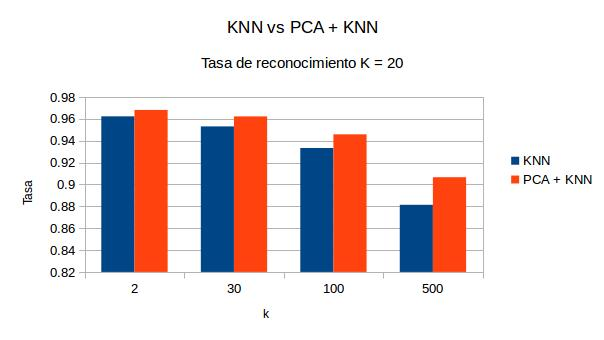
\includegraphics[scale=0.5]{Tablas/comtrK20.jpg}
}

Podemos observar como sorprendentemente PCA siempre supera a KNN, teóricamente esto no debería suceder.
\newline
\newline
A continuación presentamos un gráfico que compara los tiempos de KNN y PCA + KNN para $K = 2$ y $K = 10$, fijando $\alpha = 50$ en PCA y variando $k$:
\newline
\newline
\centerline{
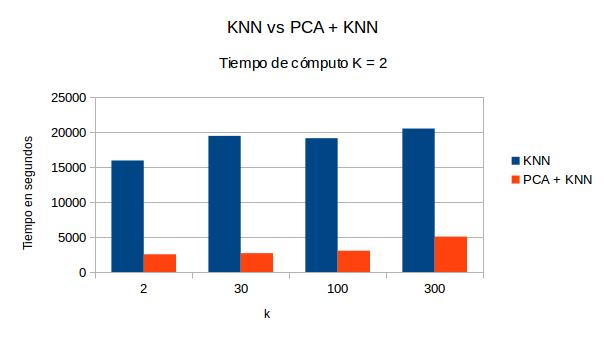
\includegraphics[scale=0.5]{Tablas/comtcK2.jpg}
}
\centerline{
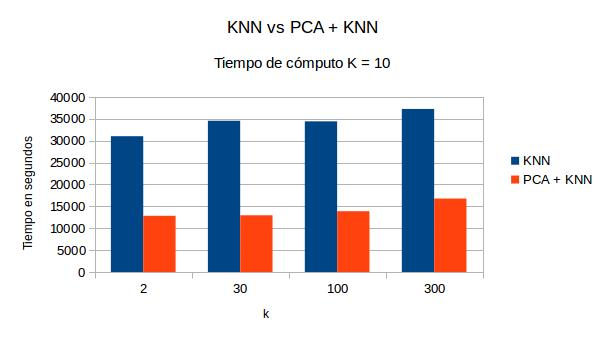
\includegraphics[scale=0.5]{Tablas/comtcK10.jpg}
}
\centerline{
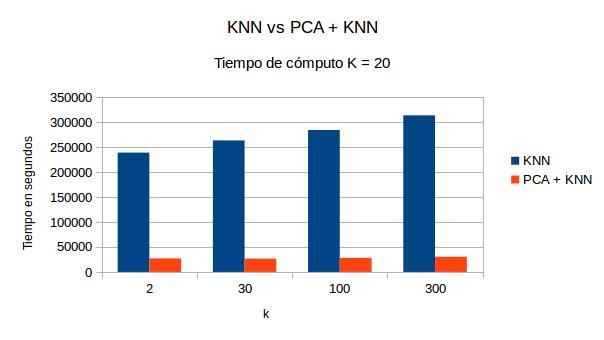
\includegraphics[scale=0.5]{Tablas/comtcK20.jpg}
}

En los gráficos muestran lo esperable que es que los tiempos de KNN son más grandes que los de PCA + KNN. Para los gráficos sobre $K = 20$, el tiempo de cómputo fue calculado de manera aproximada (multiplicando por 20 el tiempo que se tarda en procesar una partición de las 20) debido a que es demasiado grande. La tasa de reconocimiento en este caso tampoco es el promedio de las tasas porque no las tenemos, si no que es la tasa de reconocimiento de la partición particular que procesamos.

\subsubsection{Variando $\alpha$}
A continuación, presentaremos la tablas de los distintos K para los cuales corrimos PCA + KNN variando $\alpha$. En estos experimentos siempre vamos a estar utilizando el mismo valor de $k$ que va a ser 2 ya que fue elegido por ser el que maximiza la tasa de reconocimiento y minimiza el tiempo de cómputo.
\newline
\newline
\centerline{
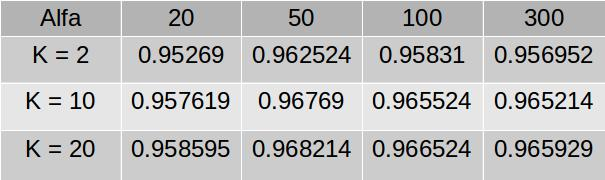
\includegraphics[scale=0.4]{Tablas/variandoAlfas.jpg}
}

Vemos como no se cumple la hipótesis que planteamos de que si aumentamos el valor de $\alpha$ entonces va a aumentar la tasa de reconocimiento ya que en los tres casos la tasa más alta está asociada a $\alpha = 50$ y es estrictamente mayor a las tasas con $\alpha = 100$ y $\alpha = 300$.
\newline Veamos los tiempos de cómputo asociados a estos valores de $\alpha$:
\newline
\newline
\centerline{
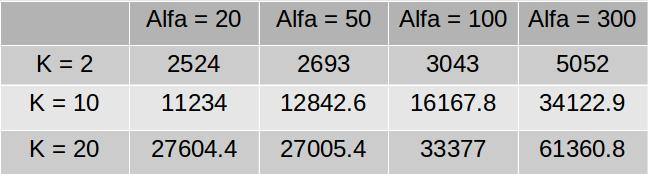
\includegraphics[scale=0.4]{Tablas/variandoalfatc.jpg}
}
\newline
\newline
Se puede ver en el gráfico como al hacer un aumento significativo en el $\alpha$ el tiempo de cómputo puede llegar a aumentar bastante. En los tres casos vemos que trabajar con $\alpha = 300$ requiere un tiempo de cómputo cercano al doble de lo que requiere con $\alpha = 20$. Esto significa que para valores cercanos de $\alpha$ el tiempo de cómputo no se va a ver afectado de manera significativa pero si realizamos aumentos grandes entonces es probable que el tiempo aumente de manera lineal.
\par Dado que nosotros queremos encontrar la mejor configuración tanto a nivel calidad de los resultados como tiempo de cómputo y vimos que las tasas variando $\alpha$ en 20, 50 100 y 300 son muy parecidas podríamos elegir $\alpha = 20$. De esta manera estaríamos minimizando el tiempo de cómputo y obteniendo una tasa de reconocimiento bastante alta. Sin embargo, en un contexto donde el tiempo de cómputo puede llegar a ser mucho más grande, por ejemplo porque estamos trabajando con un $K$ mucho mayor, porque contamos con bases de datos de mayor tamaño o por cualquier otro motivo, sería interesante poder reducir lo máximo que podamos al valor de $\alpha$. Es decir, nosotros sabemos que las tasas con $\alpha = 20, 50, 100$ y $300$ son muy similares, pero ¿cuanto más podemos disminuir $\alpha$ sin que la tasa de reconocimiento baje demasiado?. Para contestar esta pregunta decidimos disminuir el valor de $\alpha$ de una manera más drástica y ver que sucede. A continuación, se presentan las tasas de reconocimiento asociadas a los distintos $K$, para $\alpha = 5$:
\newline
\newline
\centerline{
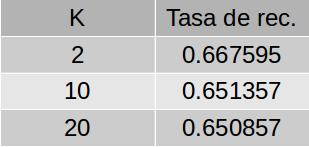
\includegraphics[scale=0.4]{Tablas/alfa5.jpg}
}
\newline
\newline
Los resultados demuestran que la diferencia de las tasas con respecto a los valores anteriores de $\alpha$ es claramente notable, lo que significa que deberíamos elegir un $\alpha$ entre 5 y 20. Es importante observar como al realizar una variación en el valor de $\alpha$, las tasas para los distintos valores de $K$ se mantienen muy parecidas. Esto significa que para reducir el tiempo de cómputo de la experimentación, podemos a tratar de encontrar este $\alpha$ utilizando $K = 2$ y lo que obtengamos también nos va a servir para $K = 10$ y $K = 20$. Probemos con $\alpha = $ 7, 13 y 16.
\newline
\newline
\centerline{
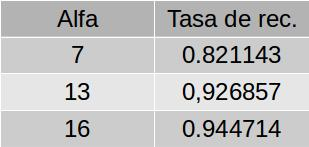
\includegraphics[scale=0.4]{Tablas/variandoalfaschicos.jpg}
}
\newline
\newline
Bien, la tabla muestra que para $\alpha = 13$ la tasa es $\approx 0.92$. Dado que con un valor de 7 estamos pasando el 0.8 y con 13 estamos pasando 0.92, tomando un valor de $\alpha = 10$ nuestra tasa va a ser $\approx 0.9$, lo cual es más que aceptable. Partimos de un valor de $\alpha = 50$ y experimentando, llegamos a que si bajamos ese valor a 10 entonces vamos a tener una tasa un poco peor pero igual muy buena y vamos a estar reduciendo mucho más la dimensión de nuestras muestras.

